\clearpage
\twocolumn[{%
\section{Detailed Analyses}
\label{app:analyses}

\subsection{The above-chance gate}
\label{app:rq00_gate_and_curves}

\noindent\begin{minipage}[t]{0.485\textwidth}
\vspace{0pt}
\paragraph{Research Question.} \emph{Which benchmarks clear chance at which size of the ladder, and which separate the language settings most?}

\paragraph{Setup.} Seed-1904 runs of every language setting, ladder and data build, 90M--1.7B. A run clears chance on a task when the one-sided 95\% Wilson lower bound of its accuracy over the task's items is above the chance level. A (task, size) cell is above chance when at least half of the runs of that size that train the task's language clear it. Tasks without a chance level (bits per byte) are not gated.
\end{minipage}\hfill
\begin{minipage}[t]{0.485\textwidth}
\vspace{0pt}
\begin{rqfinding}
\textbf{1. The gate removes most of the evaluation somewhere on the ladder.} On the 841 trained tasks, 311 (37 \%) are above chance at 90M and 507 (60 \%) at 1.7B. 547 (65 \%) are at chance at one size or more, 313 (37 \%) at every size. (Figure~\ref{fig:app_rq00_gate_and_curves}.)
\\
\\
\textbf{2. Over all 1,679 chance-level tasks the picture is the same.} 565 of 1,433 scored (39 \%) pass at 90M and 954 of 1,663 (57 \%) at 1.7B. 682 (41 \%) never pass, 16 of them never scored.
\\
\\
\textbf{3. It is an answer-format effect, not an option-count one.} On the trained languages at 1.7B the letter-answer families nearly vanish while their cloze twins pass: \texttt{belebele} 3 / 59 tasks against 57 / 59, \texttt{global\_mmlu\_full} 1 / 29 against 29 / 29, \texttt{include\_base\_44} 3 / 36 against 29 / 36.
\end{rqfinding}
\end{minipage}

\vspace{\baselineskip}
\noindent\begin{minipage}{\textwidth}
\centering
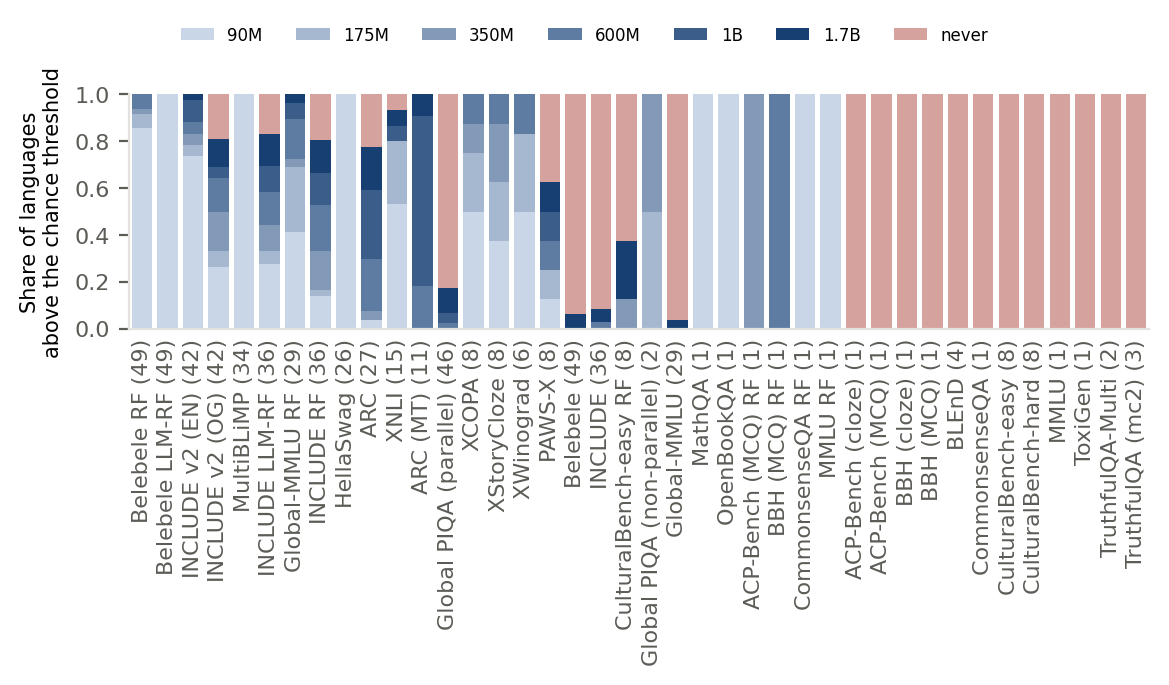
\includegraphics[width=\textwidth,height=0.36\textheight,keepaspectratio]{figures/app_rq00_chance_share_horizontal.png}
% source: src/signal-and-noise/analysis/rq00_gate_and_curves/pretraining/predictivity/first_size_share_paper_horizontal.png
\captionof{figure}{\textbf{The gate removes most of the evaluation somewhere on the ladder.} One bar per benchmark gives the share of its language tasks that clear the above-chance gate, split by the smallest model size from which the gate holds (a darker blue is a larger size). Red marks the tasks that stay at chance up to 1.7B. The number in parentheses is the benchmark's number of language tasks. The benchmarks are ordered from the most to the fewest tasks above chance.}
\label{fig:app_rq00_gate_and_curves}
\end{minipage}
\vspace{\baselineskip}
}]

\begin{table*}[p]
\centering
\small
\caption{\textbf{The tasks that pass at very small token counts answer with one option.} The ten tasks above chance in at least half of their cells below $10^{8}$ tokens of their language and in fewer than half of their cells at $10^{8}$--$10^{10}$ tokens. We read the deep runs with the baseline data at seed 1904, at every evaluated tenth, from their stored option log-likelihoods. Share of runs above chance: trained runs below $10^{8}$ tokens of the language (Low), trained runs at $10^{8}$--$10^{10}$ tokens (Mid), and runs that never trained the language nor a language of its subfamily, at the sizes and checkpoints of the Low runs (Untrained). Over the Low runs above chance: their number, the median share of items answered with the option the run picks most often (One option), and the share of these runs in which that option alone would clear chance (Constant passes). Longest option: the median share of picks on the single longest option and the share of gold answers on it. CulturalBench-easy asks in English about a country and is placed at the tokens of the country's language.}
\label{tab:app_rq00_early_passes}
\begin{tabular}{llrcccccccc}
\toprule
 & & & \multicolumn{3}{c}{Share of runs above chance} & \multicolumn{3}{c}{Passing low-token runs} & \multicolumn{2}{c}{Longest option} \\
\cmidrule(lr){4-6}\cmidrule(lr){7-9}\cmidrule(lr){10-11}
Benchmark & Lang. & Items & Low & Mid & Untrained & Runs & One option & Constant passes & Picked & Gold \\
\midrule
CulturalBench-easy (Argentina) & es & 35 & 0.79 & 0.31 & 0.88 & 11 & 0.91 & 0.91 & 0.13 & 0.23 \\
CulturalBench-easy (Chile) & es & 22 & 0.64 & 0.23 & 0.62 & 9 & 0.91 & 0.89 & 0.26 & 0.32 \\
CulturalBench-easy (India) & hi & 46 & 0.38 & 0.09 & 0.31 & 33 & 0.78 & 0.97 & 0.18 & 0.22 \\
CulturalBench-easy (Japan) & ja & 53 & 0.79 & 0.28 & 0.75 & 11 & 0.94 & 0.91 & 0.20 & 0.28 \\
CulturalBench-easy (Mexico) & es & 49 & 0.64 & 0.26 & 0.75 & 9 & 0.94 & 1.00 & 0.26 & 0.24 \\
CulturalBench-easy (Morocco) & ar & 17 & 0.45 & 0.22 & 0.42 & 32 & 0.88 & 1.00 & 0.24 & 0.18 \\
CulturalBench-easy (Peru) & es & 19 & 0.57 & 0.20 & 0.62 & 8 & 0.97 & 1.00 & 0.06 & 0.31 \\
CulturalBench-easy (Spain) & es & 40 & 0.64 & 0.27 & 0.62 & 9 & 0.95 & 1.00 & 0.27 & 0.35 \\
INCLUDE (Georgian) & ka & 500 & 0.30 & -- & 0.33 & 18 & 0.97 & 0.94 & 0.22 & 0.23 \\
PAWS-X (Japanese) & ja & 2{,}000 & 0.64 & 0.11 & 0.12 & 9 & 0.89 & 1.00 & 0.89 & 0.56 \\
\bottomrule
\end{tabular}

% source: src/signal-and-noise/analysis/rq00_gate_and_curves/pretraining/predictivity/early_passes.tex
\end{table*}

\begin{figure*}[p]
\centering
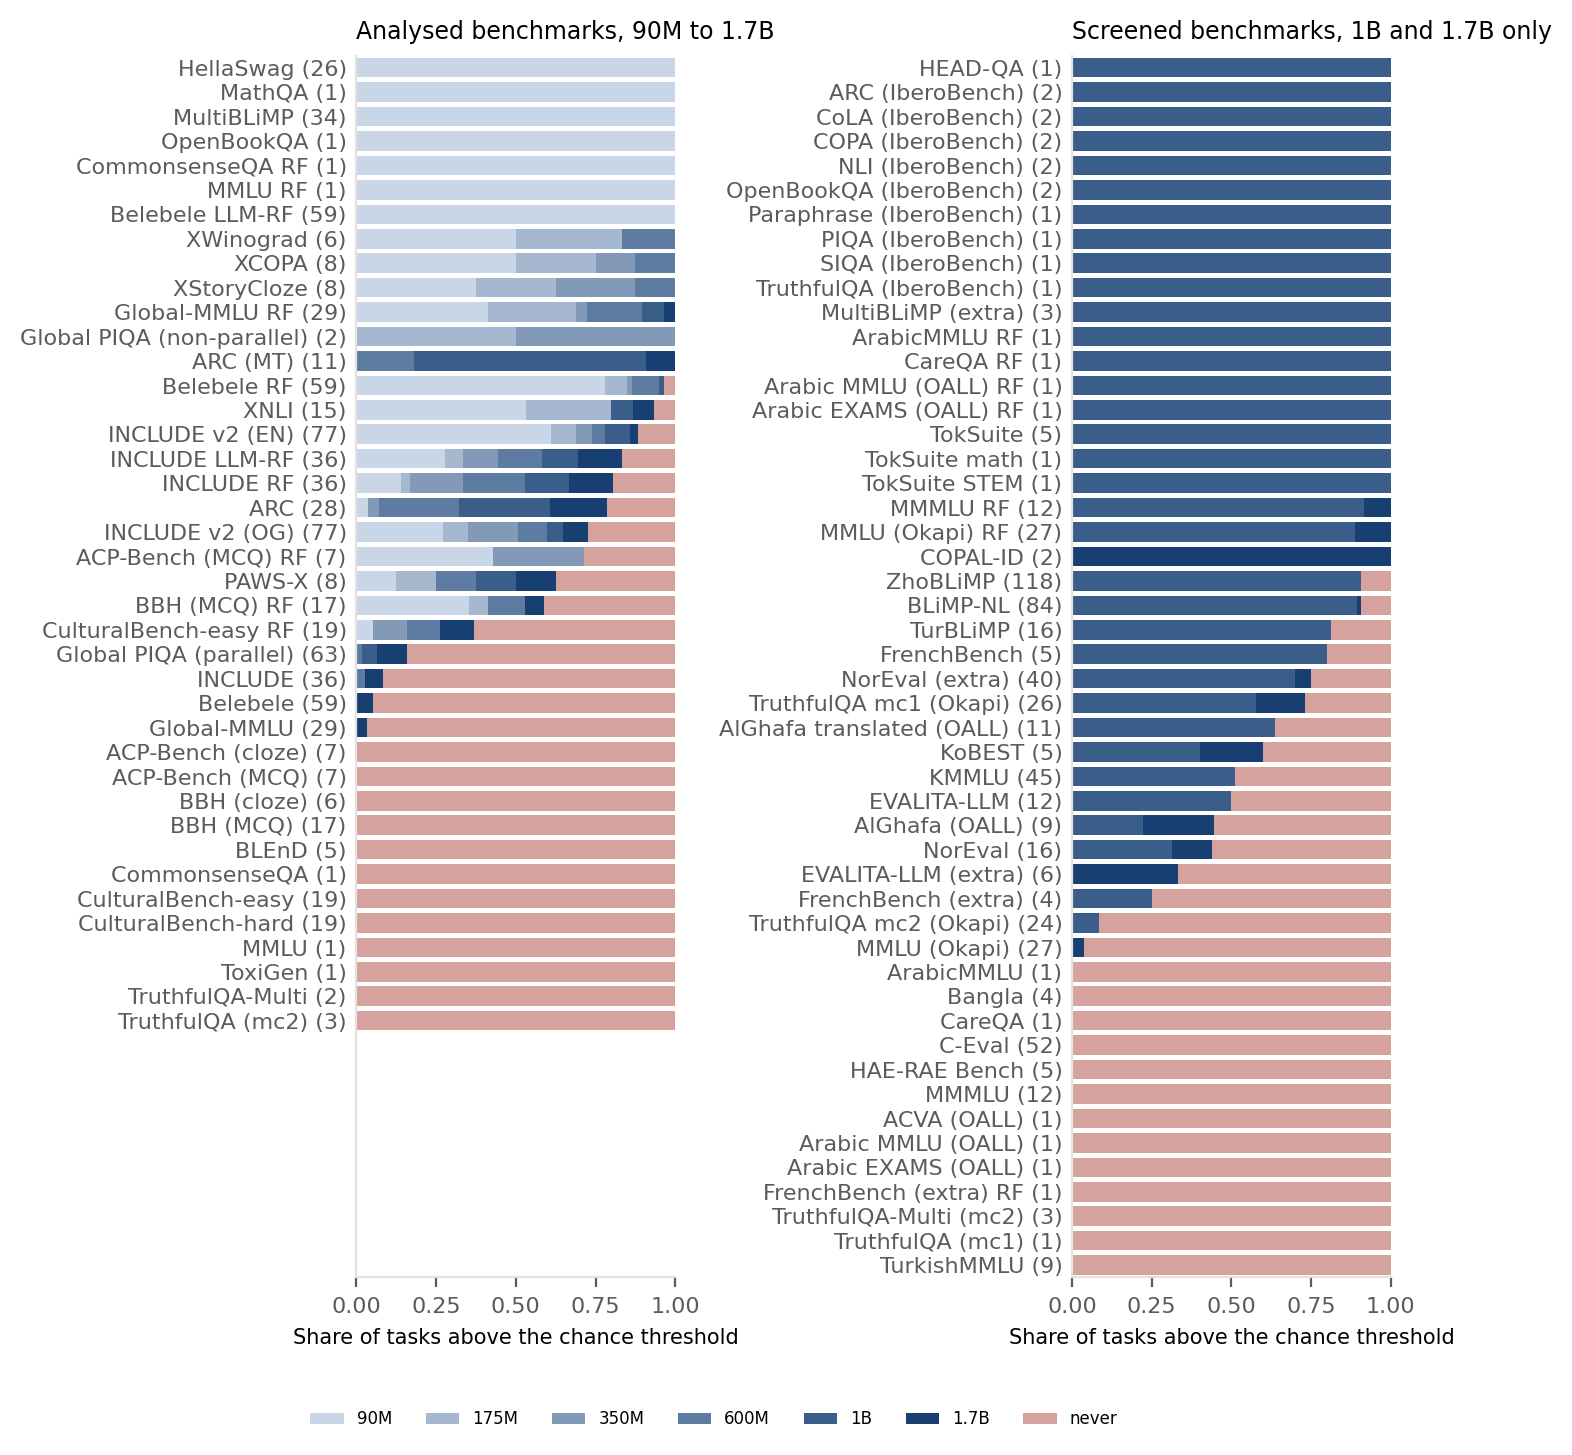
\includegraphics[width=\textwidth,height=0.8\textheight,keepaspectratio]{figures/app_rq00_chance_considered.png}
% source: src/signal-and-noise/analysis/rq00_gate_and_curves/pretraining/predictivity/first_size_share_all_considered_paper.png
\caption{\textbf{Most of the benchmarks we screened and did not adopt clear chance at 1B and 1.7B.} Left: the analysed benchmarks of Figure~\ref{fig:app_rq00_gate_and_curves}, here split by task. Right: the benchmarks we evaluated only on the final checkpoints of the 1B and 1.7B models and did not adopt, with the discarded tasks. Each bar splits a benchmark's tasks by the smallest model size from which they stay above chance (a darker blue is a larger size). On the right only 1B and 1.7B are evaluated, so 1B means above chance at both sizes. Red marks the tasks at chance at 1.7B. The number in parentheses is the benchmark's number of tasks with a chance level. Seed-1904 runs that train the task's language.}
\label{fig:app_rq00_chance_considered}
\end{figure*}

\begin{table*}[p]
\centering
\small
\caption{\textbf{Over the 90 benchmarks with a chance level that we considered, 882 of 1,451 tasks are above chance at 1.7B, and 375 of the 510 screened tasks pass although we did not adopt them.} Tasks above chance over tasks with a verdict, per group, answer format and model size, on the trained languages. Analysed is the benchmark group of every other analysis. Screened, not adopted are the benchmarks we evaluated only on the final checkpoints of the 1B and 1.7B models. Discarded are the 100 screened tasks at chance at both sizes. Original is the benchmark as published, RF scores the answer strings instead of the option letters, and LLM-RF is the LLM rewrite into statements. A cell is above chance when at least half of the seed-1904 runs of that size that train the task's language clear chance. Tasks without a chance level have no verdict.}
\label{tab:app_rq00_pass_counts_considered}
\begin{tabular}{llrrrrrrrr}
\toprule
 & & & & \multicolumn{6}{c}{Tasks above chance / tasks with a verdict} \\
\cmidrule(lr){5-10}
Group & Format & Bench. & Tasks & 90M & 175M & 350M & 600M & 1B & 1.7B \\
\midrule
Analysed & original & 30 & 577 & 166/577 & 178/577 & 202/577 & 222/577 & 253/577 & 279/577 \\
 & RF & 8 & 169 & 76/169 & 91/169 & 101/169 & 122/169 & 130/169 & 139/169 \\
 & LLM-RF & 2 & 95 & 69/95 & 71/95 & 75/95 & 80/95 & 85/95 & 89/95 \\
 & all & 40 & 841 & 311/841 & 340/841 & 378/841 & 424/841 & 468/841 & 507/841 \\
\midrule
Screened, not adopted & original & 41 & 466 & -- & -- & -- & -- & 321/466 & 332/466 \\
 & RF & 7 & 44 & -- & -- & -- & -- & 39/44 & 43/44 \\
 & all & 48 & 510 & -- & -- & -- & -- & 360/510 & 375/510 \\
\midrule
Discarded & original & 9 & 100 & -- & -- & -- & -- & 0/100 & 0/100 \\
\midrule
All considered & all & 90 & 1{,}451 & -- & -- & -- & -- & 828/1{,}451 & 882/1{,}451 \\
\bottomrule
\end{tabular}

% source: src/signal-and-noise/analysis/rq00_gate_and_curves/pretraining/predictivity/gate_pass_counts_all_considered.tex
\end{table*}
